% presentaciones/sesion03-cap03/sesion03.tex
% Sesión 3 — Capítulo 3: Gestión de datos del consumidor: valor, omnicanalidad, escucha y decisión
% Laboratorio: Gestión de datos, comportamiento y perfiles del consumidor digital
% Lic. en Mercadotecnia Digital · ESCA Unidad Santo Tomás · IPN
% Fuente de contenido: libro-consumidor-digital/partes/parte1/cap03.tex
% Figuras reutilizadas del libro (TikZ y MATLAB) sin copiarlas: ver \graphicspath y \input.
\documentclass[aspectratio=169,xcolor=dvipsnames]{beamer}
\usetheme{Berlin}

%----------------------------------------------------------------------------------------
%   PALETA INSTITUCIONAL IPN (Manual de Identidad Gráfica, Pantone 222C)
%----------------------------------------------------------------------------------------
\usepackage[dvipsnames,svgnames,x11names]{xcolor}
\definecolor{IPNguinda}{HTML}{6F1D46}       % Pantone 222C oficial — color primario
\definecolor{IPNguindaOsc}{HTML}{45102C}    % sombra / paleta secundaria
\definecolor{IPNguindaClara}{HTML}{F4E9EF}  % fondo de bloques normales
\definecolor{IPNdorado}{HTML}{B8975A}       % dorado — SOLO enlaces y detalles del cierre
\definecolor{IPNterracota}{HTML}{9C5B44}    % alertblock
\definecolor{IPNterracotaClara}{HTML}{F6ECE6}
\definecolor{IPNbronce}{HTML}{8C6B3F}       % exampleblock
\definecolor{IPNbronceClaro}{HTML}{F5F0E3}
\definecolor{IPNgris}{HTML}{58595B}         % texto secundario / notas

% Alias con los nombres de config/colores.tex del libro, para que las figuras
% TikZ del libro se puedan \input sin modificarlas
\colorlet{guindaIPN}{IPNguinda}
\colorlet{guindaIPNOsc}{IPNguindaOsc}
\colorlet{guindaIPNClara}{IPNguindaClara}
\colorlet{doradoIPN}{IPNdorado}
\colorlet{bronceIPN}{IPNbronce}
\colorlet{bronceIPNClaro}{IPNbronceClaro}
\colorlet{grisIPN}{IPNgris}
\colorlet{terracotaIPN}{IPNterracota}
\colorlet{terracotaIPNClara}{IPNterracotaClara}
\definecolor{colorLaboratorio}{HTML}{1B6E7A}

\setbeamercolor{palette primary}{bg=IPNguinda,fg=white}
\setbeamercolor{palette secondary}{bg=IPNguindaOsc,fg=white}
\setbeamercolor{palette tertiary}{bg=IPNguindaOsc,fg=white}
\setbeamercolor{palette quaternary}{bg=IPNguinda,fg=white}
\setbeamercolor{structure}{fg=IPNguinda}
\setbeamercolor{title}{bg=IPNguinda,fg=white}
\setbeamercolor{frametitle}{bg=IPNguinda,fg=white}
\setbeamercolor{block title}{bg=IPNguinda,fg=white}
\setbeamercolor{block body}{bg=IPNguindaClara,fg=black}
\setbeamercolor{block title alerted}{bg=IPNterracota,fg=white}
\setbeamercolor{block body alerted}{bg=IPNterracotaClara,fg=black}
\setbeamercolor{block title example}{bg=IPNbronce,fg=white}
\setbeamercolor{block body example}{bg=IPNbronceClaro,fg=black}
\setbeamercolor{alerted text}{fg=IPNterracota}
\setbeamercolor{item}{fg=IPNguinda}
\setbeamercolor{section in toc}{fg=IPNguinda}
\setbeamercolor{footline}{bg=IPNguindaOsc,fg=white}

\usepackage[spanish,es-noshorthands,es-nodecimaldot]{babel}
\usepackage{csquotes}
\usepackage{hyperref}
\usepackage{graphicx}
\usepackage{booktabs}
\usepackage{array}
\usepackage{amsmath}
\setbeamertemplate{caption}[numbered]
\usepackage{xurl}
\usepackage{adjustbox}
\usepackage{tikz}
\usetikzlibrary{arrows.meta,positioning}
\usepackage{pgfplots}
\pgfplotsset{compat=1.18}

\graphicspath{{Figures/}{../../libro-consumidor-digital/figuras/matlab/}}
\newcommand{\figtikz}[1]{../../libro-consumidor-digital/figuras/tikz/#1}
\newcommand{\fuente}[1]{{\tiny\color{IPNgris}Fuente: #1}}

\hypersetup{
    colorlinks=true,
    linkcolor=IPNdorado,
    filecolor=IPNguinda,
    urlcolor=IPNguinda,
    citecolor=IPNguinda,
    pdftitle={Sesion 3 - Gestion de datos del consumidor},
    pdfauthor={Dr. Aboud Barsekh-Onji},
}

%----------------------------------------------------------------------------------------
%   CODE LISTINGS — sintaxis ESTÁNDAR del lenguaje
%----------------------------------------------------------------------------------------
\usepackage{listings}
\definecolor{backcolour}{rgb}{0.97,0.97,0.99}
\definecolor{codegreen}{rgb}{0,0.6,0}

\lstdefinestyle{MATLABStyle}{
  language=Matlab,
  basicstyle=\ttfamily\scriptsize,
  keywordstyle=\color{blue}\bfseries,
  commentstyle=\color{codegreen},
  stringstyle=\color{violet},
  breaklines=true,
  numbers=left,
  numbersep=5pt,
  frame=lines,
  backgroundcolor=\color{backcolour}
}
\lstset{style=MATLABStyle}

%----------------------------------------------------------------------------------------
%   TITLE CONFIGURATION
%----------------------------------------------------------------------------------------
\logo{
\includegraphics[height=0.75cm]{ipn-escudo.png}}
\title[Sesión 3 · Gestión de datos]{Gestión de datos del consumidor: valor, omnicanalidad, escucha y decisión}
\subtitle{Sesión 3 · Unidad I — Capítulo 3}
\author{Dr. Aboud Barsekh-Onji}
\institute[IPN]{
    Instituto Politécnico Nacional \\
    \small ESCA Unidad Santo Tomás · Lic. en Mercadotecnia Digital \\
    \footnotesize Laboratorio: Gestión de datos, comportamiento y perfiles del consumidor digital
}
\date{\today}

%----------------------------------------------------------------------------------------
%   AUTO AGENDA AT EACH SECTION
%----------------------------------------------------------------------------------------
\AtBeginSection[]{
  \begin{frame}{Agenda}
    \tableofcontents[currentsection]
  \end{frame}
}


\begin{document}

\begin{frame}
    \titlepage
    \vspace{-4pt}
    \begin{center}
        {\tiny\color{IPNgris} ORCID: \href{https://orcid.org/0009-0004-5440-8092}{0009-0004-5440-8092}}
    \end{center}
\end{frame}

%------------------------------------------------
\section{Encuadre}
%------------------------------------------------

\begin{frame}{Ficha de la sesión}
\begin{columns}[T]
  \column{0.52\textwidth}
  \begin{block}{Unidad I}
    \small Comportamiento, perfil y gestión de datos del consumidor digital
  \end{block}
  \begin{block}{Temas del programa (1.3 Gestión de datos)}
    \scriptsize
    \begin{itemize}
      \item[1.3.1] Creación de valor para el consumidor-usuario (CX-UX)
      \item[1.3.2] Experiencias omnicanal consumidor-usuario (CX-UX)
      \item[1.3.3] Momentos de escucha a los consumidores digitales
      \item[1.3.4] Importancia de la recolección y gestión de datos
      \item[1.3.5] Toma de decisiones basadas en la gestión de datos digitales
    \end{itemize}
  \end{block}
  \column{0.44\textwidth}
  \begin{block}{Carga horaria}
    \small Teoría 3.0 h · Práctica 2.0 h\\ Aprendizaje autónomo 1.0 h
  \end{block}
  \begin{exampleblock}{Competencia de la unidad}
    \small Identifica el comportamiento del consumidor digital y su evolución a partir de sus tipos de perfil y gestión de datos.
  \end{exampleblock}
\end{columns}
\end{frame}

\begin{frame}{Al terminar la sesión podrás\ldots}
\begin{enumerate}
  \item \textbf{Distinguir} experiencia de cliente (CX) de experiencia de usuario (UX) y ubicarlas en el mapa de gestión de datos.
  \vspace{6pt}
  \item \textbf{Aplicar} limpieza de datos, segmentación RFM, CLV y una prueba A/B para fundamentar una decisión.
  \vspace{6pt}
  \item \textbf{Explicar} el marco legal mexicano vigente de protección de datos personales y sus implicaciones para la recolección de datos.
\end{enumerate}
\vspace{8pt}
\begin{alertblock}{Recordatorio}
  Aprendizaje autónomo de la Sesión 2: entrega a más tardar el \textbf{martes 6 de octubre}, en su carpeta del portafolio.
\end{alertblock}
\end{frame}

\begin{frame}{Arranque: ¿cuándo te \enquote{escucha} una marca?}
\begin{columns}[T]
  \column{0.55\textwidth}
  \begin{exampleblock}{Pregunta de arranque}
    Piensen en la última compra en línea que \textbf{abandonaron} a medias.\\[4pt]
    ¿Se lo dijeron a alguien? ¿Cómo creen que la tienda \textbf{se enteró} (o no) de que se fueron?
  \end{exampleblock}
  \vspace{4pt}
  {\small\color{IPNgris} Puente con la Sesión 2: el perfil depende de qué comportamiento se mide.}
  \column{0.41\textwidth}
  \begin{block}{Dinámica (10 min)}
    \small
    \begin{enumerate}
      \item Individual: anoten el paso exacto donde abandonaron (2 min).
      \item Parejas: ¿fue por precio, por un trámite o por desconfianza?
      \item Pizarrón: lista de \enquote{pasos que espantan}. Vuelve en el caso de apertura.
    \end{enumerate}
  \end{block}
\end{columns}
\end{frame}

%------------------------------------------------
\section[Apertura]{Caso de apertura}
%------------------------------------------------

\begin{frame}{La cadena de farmacias y el segundo teléfono}
\begin{exampleblock}{Caso}
  Una cadena de farmacias mexicana descubre, al revisar sus datos de fidelidad, que el \textbf{60\,\%} de quienes abandonan su carrito en la app lo hacen \textbf{en el mismo paso}: la solicitud de un segundo número telefónico para verificación en dos pasos.
\end{exampleblock}
\begin{itemize}
  \item Nadie diseñó ese paso para espantar clientes: se agregó \textbf{por seguridad} y se probó internamente.
  \item El problema es \textbf{invisible al ojo humano}: solo aparece porque la organización recolecta y analiza el comportamiento.
\end{itemize}
\vspace{2pt}
\begin{alertblock}{La tesis de la sesión}
  Los datos son una \textbf{cadena}: cómo se recolectan, qué los vuelve confiables, cómo se escucha a través de ellos y qué obligaciones legales trae tenerlos.
\end{alertblock}
\end{frame}

%------------------------------------------------
\section[CX-UX]{1.3.1--1.3.2 Valor y omnicanalidad}
%------------------------------------------------

\begin{frame}{El mapa de la gestión de datos}
\begin{center}
  \resizebox{\linewidth}{!}{\input{\figtikz{cap03-mapa-gestion-datos}}}
\end{center}
\vspace{4pt}
\begin{itemize}
  \small
  \item Recolección $\to$ limpieza $\to$ escucha $\to$ creación de valor $\to$ decisión.
  \item La \textbf{base legal} no es un paso más: es condición de \textbf{todo} el mapa.
\end{itemize}
\fuente{elaboración propia.}
\end{frame}

\begin{frame}{CX no es UX}
\begin{columns}[T]
  \column{0.48\textwidth}
  \begin{block}{UX (\textit{user experience})}
    \small El diseño de la interacción con un producto o interfaz \textbf{específicos}: qué tan fácil es completar una tarea en una app.
  \end{block}
  \column{0.48\textwidth}
  \begin{exampleblock}{CX (\textit{customer experience})}
    \small La \textbf{suma} de todas las interacciones de una persona con una organización, a lo largo del tiempo y de los canales. UX es una parte, no el todo.
  \end{exampleblock}
\end{columns}
\vspace{6pt}
\begin{alertblock}{Error común}
  Optimizar la interfaz (UX impecable) mientras el servicio detrás de la app es lento (CX deficiente) y \textbf{ningún panel lo está midiendo}.
\end{alertblock}
\fuente{Hoyer, MacInnis y Pieters (2024).}
\end{frame}

\begin{frame}{Omnicanalidad: una sola identidad de cliente}
\begin{block}{Verhoef, Kannan e Inman (2015)}
  \small La \textbf{gestión sinérgica} de los múltiples canales y puntos de contacto, de forma que la experiencia y el desempeño \textbf{a través de los canales} se optimicen.
\end{block}
\begin{center}
  \resizebox{!}{0.34\textheight}{\input{\figtikz{cap03-omnicanal}}}
\end{center}
\begin{itemize}
  \scriptsize
  \item Multicanalidad = estar en varios canales. Omnicanalidad = que compartan \textbf{una identidad} reconocible.
  \item Unificar el rastro de una persona entre canales es, por definición, \textbf{tratamiento de datos personales}.
\end{itemize}
\fuente{elaboración propia con base en Verhoef et al. (2015).}
\end{frame}

%------------------------------------------------
\section[Escucha]{1.3.3 Momentos de escucha}
%------------------------------------------------

\begin{frame}{Tres señales para escuchar al consumidor}
\begin{columns}[T]
  \column{0.31\textwidth}
  \begin{block}{Declarada}
    \small Lo que dice: reseña, encuesta, comentario en redes.
  \end{block}
  \column{0.31\textwidth}
  \begin{exampleblock}{Conductual}
    \small Lo que hace: qué compra, dónde se detiene, qué abandona.
  \end{exampleblock}
  \column{0.31\textwidth}
  \begin{block}{De contexto}
    \small Circunstancias: hora, canal, dispositivo.
  \end{block}
\end{columns}
\vspace{8pt}
\begin{alertblock}{El caso de la farmacia es escucha puramente conductual}
  Nadie tuvo que quejarse del segundo teléfono. Un programa que solo atiende lo \textbf{declarado} subestima los problemas silenciosos: la mayoría de quienes abandonan \textbf{no se queja, simplemente se va}.
\end{alertblock}
\end{frame}

%------------------------------------------------
\section[Datos y ley]{1.3.4 Recolección de datos y marco legal}
%------------------------------------------------

\begin{frame}{Datos de primera y de cero parte}
\begin{columns}[T]
  \column{0.48\textwidth}
  \begin{block}{Primera parte}
    \small Los que la organización recolecta \textbf{directamente} de su relación con el consumidor: compras, registro, navegación en su propio sitio.
  \end{block}
  \column{0.48\textwidth}
  \begin{exampleblock}{Cero parte}
    \small Los que el consumidor \textbf{entrega voluntaria y explícitamente}: encuesta de preferencias, cuestionario de talla.
  \end{exampleblock}
\end{columns}
\vspace{6pt}
\begin{itemize}
  \small
  \item Ganaron relevancia por presión regulatoria y por el supuesto fin de las cookies de terceros.
  \item Razón de fondo: \textbf{confianza} del consumidor y \textbf{cumplimiento legal}, no solo técnica.
\end{itemize}
\end{frame}

\begin{frame}{Frontera: el mito del fin de las cookies de terceros}
\begin{alertblock}{Lo que se anunció no ocurrió así}
  \small Google \textbf{revirtió en 2024} su plan de retirar las cookies de terceros en Chrome, descartó el \textit{choice prompt} en abril de 2025 y retiró las APIs de reemplazo de Privacy Sandbox en octubre de 2025.
\end{alertblock}
\begin{block}{Vigente a septiembre de 2026}
  \small Las cookies de terceros siguen activas \textbf{por defecto} en Chrome.
\end{block}
\begin{center}
  El giro a datos de primera y cero parte sigue siendo correcto,\\
  pero evita repetir que \enquote{las cookies ya desaparecieron}: \textbf{no es un hecho verificable}.
\end{center}
\fuente{European Parliamentary Research Service (2025).}
\end{frame}

\begin{frame}{México: la nueva LFPDPPP (cronología verificada)}
\small
\begin{center}
\begin{tabular}{@{}>{\raggedright}p{2.2cm}>{\raggedright\arraybackslash}p{9.6cm}@{}}
\toprule
\textbf{Fecha} & \textbf{Hecho jurídico} \\
\midrule
20-dic-2024 & Reforma constitucional de simplificación orgánica: desaparece el INAI, entre otros seis organismos autónomos. \\
20-mar-2025 & Se publica en el DOF la nueva LFPDPPP, que abroga la de 2010; \textbf{entra en vigor el 21 de marzo}. \\
9-may-2025 & Entrega-recepción del INAI a la Secretaría Anticorrupción y Buen Gobierno, que asume la protección de datos de particulares. \\
14-nov-2025 & Reforma de homologación normativa a la LFPDPPP. \\
\bottomrule
\end{tabular}
\end{center}
\fuente{DOF y comunicados oficiales de gob.mx.}
\end{frame}

\begin{frame}{Una tensión que no resolvemos}
\begin{alertblock}{Cautela deliberada}
  \small Según fuentes de análisis jurídico corporativo, la nueva ley establecería el \textbf{consentimiento tácito} como regla general (salvo datos sensibles) y, a la vez, exigiría que el consentimiento sea \textbf{libre, específico e informado}.
\end{alertblock}
\begin{block}{Qué hacer con esto}
  \small
  \begin{itemize}
    \item No se resolvió contra el \textbf{texto legal completo}: afirmarlo con firmeza sería una afirmación jurídica no sustentada.
    \item Consulten el texto vigente (reporte de indagación documental) y, para una decisión profesional real, a un \textbf{especialista}.
  \end{itemize}
\end{block}
\end{frame}

%------------------------------------------------
\section[Decisión]{1.3.5 Decisiones basadas en datos}
%------------------------------------------------

\begin{frame}{Del dato a la decisión, sin engañarse}
\begin{block}{Mercadotecnia impulsada por datos (\textit{data-driven})}
  \small Un dato limpio, bien recolectado y con base legal es \textbf{necesario}, no \textbf{suficiente}: hace falta un método que traduzca el dato en decisión.
\end{block}
\begin{center}
\begin{tabular}{@{}clp{6.4cm}@{}}
  \textbf{1} & Limpiar & antes de usar los datos \\
  \textbf{2} & Segmentar por valor (RFM, CLV) & saber \emph{a quién} dirigir el esfuerzo \\
  \textbf{3} & Probar con un experimento (A/B) & en vez de decidir por intuición \\
\end{tabular}
\end{center}
\begin{alertblock}{La forma más común de autoengaño}
  Comparar dos porcentajes en un panel y declarar ganador, \textbf{sin preguntarse si fue suerte}.
\end{alertblock}
\fuente{Kotler, Kartajaya y Setiawan (2021).}
\end{frame}

%------------------------------------------------
\section[Evidencia]{Evidencia de México}
%------------------------------------------------

\begin{frame}{Gestión de la información financiera personal (ENIF 2024)}
\begin{columns}[c]
  \column{0.55\textwidth}
  \begin{tikzpicture}
    \begin{axis}[
        width=\linewidth, height=4.2cm,
        ybar, bar width=22pt, ymin=0, ymax=100,
        symbolic x coords={Mujeres,Hombres},
        xtick=data, ylabel={\% con producto financiero formal},
        label style={font=\scriptsize}, tick label style={font=\scriptsize},
        nodes near coords, nodes near coords style={font=\scriptsize},
        enlarge x limits=0.5, axis lines*=left, ymajorgrids, grid style={IPNgris!25},
      ]
      \addplot[fill=IPNguinda, draw=IPNguindaOsc] coordinates {(Mujeres,72.8) (Hombres,80.9)};
    \end{axis}
  \end{tikzpicture}
  \column{0.41\textwidth}
  \begin{block}{Indicadores 2024}
    \small
    \begin{tabular}{@{}lr@{}}
      Con producto financiero formal & 76.5\,\% \\
      Llevan registro de sus gastos & 65.3\,\% \\
      Brecha de género & 8.1 pp \\
    \end{tabular}
  \end{block}
  \fuente{INEGI/CNBV, ENIF 2024, Comunicado 49/25.}
\end{columns}
\vspace{4pt}
\begin{alertblock}{Por qué importa para este capítulo}
  \footnotesize Una segmentación por comportamiento financiero que no pondere esta brecha puede definir \enquote{cliente de alto valor} \textbf{subrepresentando a las mujeres} sin que ningún paso lo haga explícito.
\end{alertblock}
\end{frame}

%------------------------------------------------
\section[Laboratorio]{Laboratorio MATLAB}
%------------------------------------------------

\begin{frame}{Laboratorio: RFM, CLV y prueba A/B}
\begin{block}{Objetivo}
  Limpiar datos de compras con faltantes y atípicos, segmentar clientes con \textbf{RFM}, calcular un \textbf{CLV} simple y decidir entre dos versiones de un \textit{checkout} con una \textbf{prueba A/B}: ¿B es mejor o fue suerte?
\end{block}
\begin{columns}[T]
  \column{0.48\textwidth}
  \begin{exampleblock}{CLV (valor de vida del cliente)}
    \small
    \[ \mathrm{CLV} = \text{monto} \times \text{frecuencia} \times \text{años} \]
    \scriptsize ¿Cuánto dinero dejará este cliente? Es una aproximación didáctica: sin descuento ni probabilidad de que se vaya.
  \end{exampleblock}
  \column{0.48\textwidth}
  \begin{block}{Prueba A/B}
    \small Dos versiones, dos grupos de visitantes, una pregunta: \textbf{¿la diferencia que vemos es real o la produjo el azar?}\\[3pt]
    \scriptsize El script la calcula con una fórmula (estadístico $z$); aquí la entendemos \textbf{simulando el azar}.
  \end{block}
\end{columns}
\end{frame}

\begin{frame}{Bloque 1 y 2: limpiar y segmentar}
\begin{columns}[T]
  \column{0.48\textwidth}
  \begin{block}{1. Calidad de datos}
    \scriptsize
    \begin{itemize}
      \item \textbf{Faltantes} (5\,\% de los montos): imputación por \textbf{mediana}, regla documentada.
      \item \textbf{Atípicos} (2\,\%): regla $Q_3+1.5\times\mathrm{RIC}$; se \textbf{acotan}, no se borran: se conserva su recencia y frecuencia.
    \end{itemize}
  \end{block}
  \column{0.48\textwidth}
  \begin{exampleblock}{2. RFM por quintiles}
    \scriptsize
    Puntaje 1--5 en \textbf{R}ecencia, \textbf{F}recuencia y \textbf{M}onto; suma de 3 a 15:\\[2pt]
    \begin{tabular}{@{}ll@{}}
      $\geq 12$ & Campeón \\
      9--11 & Leal \\
      6--8 & En riesgo \\
      $<6$ & Perdido \\
    \end{tabular}
  \end{exampleblock}
\end{columns}
\vspace{4pt}
\begin{alertblock}{Ojo}
  \small Los quintiles son \textbf{relativos a la propia base}: un \enquote{Campeón} es el mejor de \textit{su} base, no un cliente excelente en términos absolutos.
\end{alertblock}
\end{frame}

\begin{frame}[fragile]{El script: \texttt{cap03\_rfm\_clv\_ab.m}}
\begin{columns}[T]
  \column{0.58\textwidth}
\begin{lstlisting}[basicstyle=\ttfamily\scriptsize]
%% ==================================
%  PARAMETROS: UNICA SECCION QUE
%  EL ESTUDIANTE DEBE EDITAR
%  ==================================
nClientes = 300;     % base sintetica
horizonteAnios = 3;  % horizonte del CLV
alfa = 0.05;         % significancia A/B
nA = 1200; conversionesA = 132;  % A
nB = 1180; conversionesB = 159;  % B
\end{lstlisting}
  \column{0.38\textwidth}
  \begin{block}{Reglas y rangos}
    \scriptsize
    \begin{itemize}
      \item \texttt{alfa} = \enquote{umbral de duda}: entre 0 y 1; usuales 0.01, 0.05, 0.10.
      \item Conversiones $\leq$ visitantes.
      \item Datos \textbf{sintéticos} (\texttt{rng(42)}); el resto del script no se toca.
    \end{itemize}
  \end{block}
  \begin{exampleblock}{Sin MATLAB}
    \scriptsize \texttt{cap03\_rfm\_clv\_ab\_\allowbreak interactivo.html}: mismos parámetros y casos A, B, C.
  \end{exampleblock}
\end{columns}
\end{frame}

\begin{frame}{Salida: segmentos RFM y CLV}
\begin{center}
  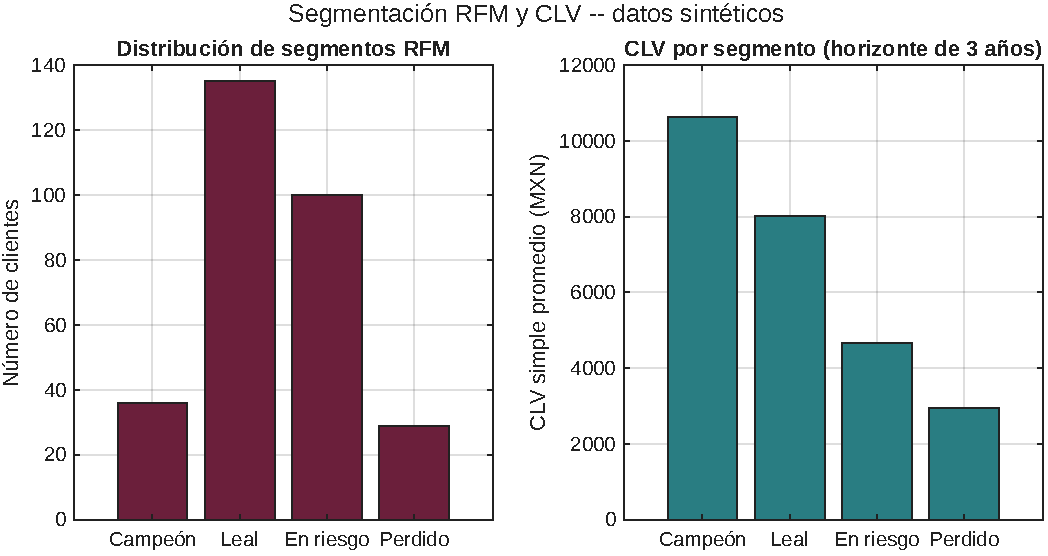
\includegraphics[width=\linewidth,height=0.58\textheight,keepaspectratio]{cap03_rfm_clv.pdf}
\end{center}
\vspace{-4pt}
\begin{center}
  \small CLV simple promedio: Campeón \textbf{\$10{,}631} · Leal \textbf{\$8{,}015} · En riesgo \textbf{\$4{,}675} · Perdido \textbf{\$2{,}957}
\end{center}
\fuente{elaboración propia, MATLAB, datos sintéticos, \texttt{rng(42)}.}
\end{frame}

\begin{frame}{Prueba A/B: ¿mejor o suerte?}
\begin{columns}[T]
  \column{0.46\textwidth}
  \begin{exampleblock}{La moneda}
    \footnotesize Lanzas una moneda 10 veces y salen 6 caras. ¿Está cargada? \textbf{No lo concluyes}: el azar siempre mueve los números.\\[3pt]
    Con A/B pasa igual: B convirtió un poco más, pero ¿es \textbf{más de lo que el azar produce solo}?
  \end{exampleblock}
  \column{0.50\textwidth}
  \begin{block}{Tres pasos}
    \footnotesize
    \begin{enumerate}
      \item \textbf{Medimos} la diferencia: B 13.5\,\% contra A 11.0\,\% $\Rightarrow$ \textbf{+2.5 puntos}.
      \item \textbf{Simulamos el azar}: imaginamos que A y B son \textbf{iguales} y repetimos el experimento 5{,}000 veces en la computadora.
      \item \textbf{Comparamos}: ¿en cuántas repeticiones el azar solo iguala o supera esos 2.5 puntos?
    \end{enumerate}
  \end{block}
\end{columns}
\vspace{4pt}
\begin{alertblock}{Cómo se decide}
  \footnotesize Menos de \textbf{5 de cada 100} $\Rightarrow$ diferencia \textbf{confiable}. Más seguido $\Rightarrow$ \textbf{todavía no se puede saber} (no significa que sean iguales: falta información).
\end{alertblock}
\end{frame}

\begin{frame}{El azar sí llega a 2.5 puntos}
\begin{columns}[c]
  \column{0.56\textwidth}
  \begin{tikzpicture}
    \begin{axis}[
        width=\linewidth, height=5.2cm, ymin=0, ymax=450, xmin=-5, xmax=5, xtick={-4,-2,0,2,4},
        xlabel={\scriptsize diferencia B $-$ A por puro azar (puntos)}, ylabel={\scriptsize experimentos (de 5{,}000)},
        label style={font=\scriptsize}, tick label style={font=\scriptsize},
        axis lines*=left, ymajorgrids, grid style={IPNgris!25}, enlarge x limits=0.02,
      ]
      \addplot[ycomb, line width=4.2pt, color=IPNgris!55] coordinates {(-2.125,105) (-1.875,144) (-1.625,162) (-1.375,211) (-1.125,278) (-0.875,297) (-0.625,337) (-0.375,350) (-0.125,370) (0.125,363) (0.375,349) (0.625,343) (0.875,319) (1.125,242) (1.375,227) (1.625,190) (1.875,119) (2.125,111)};
      \addplot[ycomb, line width=4.2pt, color=IPNterracota] coordinates {(-4.375,1) (-4.125,1) (-3.875,1) (-3.625,11) (-3.375,18) (-3.125,22) (-2.875,54) (-2.625,54) (-2.375,71) (2.375,81) (2.625,61) (2.875,47) (3.125,25) (3.375,13) (3.625,9) (3.875,8) (4.125,3) (4.375,1) (4.625,1) (4.875,1)};
      \draw[IPNdorado, very thick] (axis cs:2.47,0) -- (axis cs:2.47,430) node[right, font=\tiny, text=IPNbronce]{lo medido};
    \end{axis}
  \end{tikzpicture}
  \column{0.40\textwidth}
  \begin{block}{Lectura}
    \small En \textbf{6.5 de cada 100} experimentos de solo azar sale una diferencia igual o mayor (en rojo): arriba del umbral de 5.
  \end{block}
  \begin{alertblock}{Veredicto}
    \small \textbf{Todavía no se puede saber.} Para estar seguros de una diferencia así harían falta $\approx$\textbf{2{,}750} visitantes por versión; hay 1{,}200.
  \end{alertblock}
\end{columns}
\fuente{elaboración propia; simulación con datos sintéticos del Caso A. El 6.5 es el valor $p$ del script ($z=1.84$).}
\end{frame}

\begin{frame}{La prueba A/B en la gráfica del script}
\begin{columns}[c]
  \column{0.44\textwidth}
  \centering
  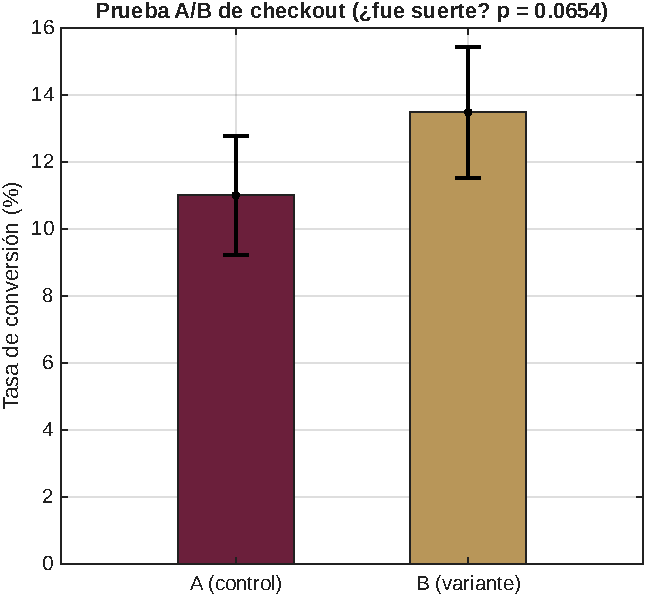
\includegraphics[width=\linewidth,height=0.66\textheight,keepaspectratio]{cap03_prueba_ab.pdf}
  \column{0.52\textwidth}
  \begin{block}{Cómo leerla}
    \small Cada barra es la conversión; las rayitas son el \textbf{margen de error}. Si se \textbf{traslapan} mucho, desconfía de la diferencia.
  \end{block}
  \begin{alertblock}{Decidir \enquote{por el ojo}}
    \small Ver diferencia donde solo hay ruido es la \textbf{heurística de representatividad} (Tversky y Kahneman, 1974).
  \end{alertblock}
  \begin{exampleblock}{La decisión correcta}
    \small No \enquote{B es mejor} ni \enquote{no importa}: \textbf{seguir la prueba} con más tráfico.
  \end{exampleblock}
\end{columns}
\end{frame}

\begin{frame}{Ejercicio propuesto: tres corridas}
\begin{columns}[T]
  \column{0.46\textwidth}
  \begin{exampleblock}{Casos (solo el bloque de parámetros)}
    \scriptsize
    \begin{itemize}
      \item[\textbf{A}] Valores por defecto: $n_A=1200$, 132 compras; $n_B=1180$, 159; umbral de duda $\alpha=0.05$.
      \item[\textbf{B}] Mismas tasas, \textbf{5 veces más visitantes}: $n_A=6000$, 660; $n_B=5900$, 795.
      \item[\textbf{C}] Datos del Caso A con umbral $\alpha=0.10$ (aceptas más suerte).
    \end{itemize}
  \end{exampleblock}
  \column{0.50\textwidth}
  \footnotesize
  \begin{tabular}{@{}lccc@{}}
    \toprule
    Caso & Conv. A / B & ¿Fue suerte? ($p$) & Veredicto \\
    \midrule
    A & \rule{0.9cm}{0.4pt} & \rule{0.9cm}{0.4pt} & \rule{1.1cm}{0.4pt} \\[2pt]
    B & \rule{0.9cm}{0.4pt} & \rule{0.9cm}{0.4pt} & \rule{1.1cm}{0.4pt} \\[2pt]
    C & \rule{0.9cm}{0.4pt} & \rule{0.9cm}{0.4pt} & \rule{1.1cm}{0.4pt} \\
    \bottomrule
  \end{tabular}
  \vspace{2pt}
  \begin{block}{Respondan con sus corridas}
    \scriptsize
    \begin{enumerate}
      \item Las tasas son las mismas en A y B (11\,\% y 13.5\,\%): ¿por qué cambia el veredicto con más visitantes?
      \item ¿Cambia el veredicto de A a C? ¿Qué riesgo corres al aceptar más suerte (\enquote{falsa alarma})?
      \item ¿En qué negocios sería aceptable correr ese riesgo?
    \end{enumerate}
  \end{block}
\end{columns}
\end{frame}

\begin{frame}{Práctica con sus propios datos: app HTML}
\begin{columns}[T]
  \column{0.52\textwidth}
  \begin{block}{\texttt{cap03\_rfm\_datos\_propios.html}}
    \small Sin MATLAB y sin conexión: suban un Excel con \textbf{recencia, frecuencia y monto} de sus clientes (y, opcional, su experimento A/B) y recorran cinco pasos:
    \scriptsize
    \begin{enumerate}
      \item Calidad de datos y reglas de limpieza.
      \item Segmentación RFM y qué hacer con cada segmento.
      \item CLV (con periodo y tasa de descuento).
      \item Prueba A/B: simulación del azar y visitantes necesarios.
      \item Lectura de negocio y descarga en Excel.
    \end{enumerate}
  \end{block}
  \column{0.44\textwidth}
  \begin{exampleblock}{Reglas del archivo}
    \scriptsize
    \begin{itemize}
      \item Hoja \texttt{Datos}: una fila por cliente, encabezados en la fila 1.
      \item Hoja \texttt{Experimento} (opcional): \texttt{Version} y \texttt{Convirtio}.
      \item \textbf{Sin} nombres, correos ni teléfonos: ID anónimo.
      \item Sus datos \textbf{no salen} de su computadora.
    \end{itemize}
  \end{exampleblock}
\end{columns}
\end{frame}

\begin{frame}{Ética: segmentar y contactar es tratar datos personales}
\begin{alertblock}{La pregunta de fondo}
  ¿Con qué \textbf{base legal} y \textbf{propósito declarado} puedo usar el RFM de un cliente real para contactarlo?
\end{alertblock}
\begin{block}{Como mínimo}
  \begin{itemize}
    \item Verificar la \textbf{LFPDPPP vigente} al implementar, no solo al estudiar: hubo reforma en noviembre de 2025 y es razonable esperar más.
    \item Ninguna decisión de recolección (identidad omnicanal, RFM, consentimiento) debe basarse en este curso como \textbf{fuente única}.
  \end{itemize}
\end{block}
\end{frame}

%------------------------------------------------
\section[Caso]{Estudio de caso}
%------------------------------------------------

\begin{frame}{Caso: la plataforma de cursos en línea}
\begin{exampleblock}{Caso ficticio}
  Una plataforma nota que la finalización de sus cursos gratuitos es de \textbf{8\,\%}. Prueba un rediseño del panel de progreso (barra de avance más visible, recordatorios por correo) durante dos semanas con \textbf{400 estudiantes por grupo}.
\end{exampleblock}
\begin{columns}[T]
  \column{0.48\textwidth}
  \begin{block}{Resultado}
    \small Control: \textbf{8.5\,\%}\\ Rediseño: \textbf{11\,\%}
  \end{block}
  \column{0.48\textwidth}
  \begin{alertblock}{Lo que dice producto}
    \small \enquote{El rediseño aumenta la finalización 3 puntos porcentuales: hay que lanzarlo a todos.}
  \end{alertblock}
\end{columns}
\end{frame}

\begin{frame}{Preguntas guía}
\small
\begin{enumerate}
  \item Con 400 y 400 estudiantes y 11\,\% y 8.5\,\%, use la app del laboratorio (Caso A/B con esos datos): ¿la diferencia es \textbf{confiable} o \textbf{todavía no se sabe}?
  \vspace{3pt}
  \item Si no lo fuera, ¿qué le respondería al equipo de producto que quiere lanzar de inmediato?
  \vspace{3pt}
  \item ¿Qué otros datos, además de la tasa de finalización, ayudarían a decidir si vale el costo de desarrollo, aun con una diferencia confiable?
  \vspace{3pt}
  \item Relacionen el caso con la señal declarada y la conductual: ¿en qué categoría cae la tasa de finalización?
\end{enumerate}
\begin{alertblock}{Entregable}
  \small Solución escrita con las cuatro preguntas respondidas.
\end{alertblock}
\end{frame}

%------------------------------------------------
\section{Cierre}
%------------------------------------------------

\begin{frame}{Síntesis: la cadena del dato}
\begin{itemize}
  \footnotesize
  \item La gestión de datos es una \textbf{cadena}: recolección, limpieza, escucha, valor y decisión, con la \textbf{base legal} como condición transversal.
  \item \textbf{CX $\neq$ UX}; la omnicanalidad exige una identidad única de cliente: tarea técnica \textbf{y} legal.
  \item El marco mexicano cambió de fondo en 2025, con una \textbf{tensión normativa} (consentimiento tácito frente a informado) que no se resuelve sin el texto legal.
  \item Ninguna decisión basada en datos es mejor que el \textbf{rigor del método}: comparar porcentajes sin preguntarse si es suerte es el autoengaño más común.
\end{itemize}
\vspace{4pt}
\begin{center}
  \resizebox{!}{0.27\textheight}{\input{\figtikz{parte1-infografia-perfil}}}
\end{center}
\end{frame}

\begin{frame}{Autoevaluación rápida}
\footnotesize
\begin{enumerate}
  \item La diferencia central entre CX y UX es que:
  \begin{itemize}
    \item[a)] son sinónimos intercambiables;
    \item[b)] \alt<2->{\textcolor{IPNguinda}{\textbf{UX es el diseño de una interacción específica; CX es la suma de todas las interacciones en el tiempo y los canales}}}{UX es el diseño de una interacción específica; CX es la suma de todas las interacciones en el tiempo y los canales};
    \item[c)] CX aplica solo a apps móviles.
  \end{itemize}
  \item La nueva LFPDPPP entró en vigor:
  \begin{itemize}
    \item[a)] el 20 de diciembre de 2024;
    \item[b)] \alt<2->{\textcolor{IPNguinda}{\textbf{el 21 de marzo de 2025}}}{el 21 de marzo de 2025};
    \item[c)] el 14 de noviembre de 2025.
  \end{itemize}
  \item En el laboratorio, el azar solo iguala la diferencia observada en 6.5 de cada 100 simulaciones y tu umbral de duda es 5 de cada 100. Entonces:
  \begin{itemize}
    \item[a)] la versión B es definitivamente mejor;
    \item[b)] \alt<2->{\textcolor{IPNguinda}{\textbf{todavía no se puede saber si B es mejor: falta información}}}{todavía no se puede saber si B es mejor: falta información};
    \item[c)] el experimento falló y debe descartarse.
  \end{itemize}
\end{enumerate}
\end{frame}

\begin{frame}{Evidencias del portafolio}
\begin{block}{Pasos para subir los trabajos al portafolio}
    \begin{itemize}
    \item Accede a esta carpeta de evidencia: \url{https://drive.google.com/drive/folders/1sr_SAVkl_Mjil6ZRWz3O2mveMoZVW6cp?usp=sharing}
    \item Crea una carpeta con tu nombre y organiza en ella todos tus entregables del semestre.
    \item Considera los tiempos límite establecidos para cada actividad.
    \end{itemize}
  \end{block}
\end{frame}

\begin{frame}{Evidencias del portafolio}
\small
\begin{columns}[T]
  \column{0.48\textwidth}
  \begin{block}{Reporte de indagación documental}
    \scriptsize Consultar el texto vigente de la LFPDPPP (Secretaría Anticorrupción y Buen Gobierno) y resumir, con cita textual de máximo 40 palabras, el artículo sobre el consentimiento.
  \end{block}
  \begin{block}{Exposición}
    \scriptsize CX frente a UX con un ejemplo real de una organización mexicana donde una esté mejor atendida que la otra.
  \end{block}
  \begin{block}{Solución de casos}
    \scriptsize Caso de la plataforma de cursos, con la corrida de la app y su interpretación.
  \end{block}
  \column{0.48\textwidth}
  \begin{block}{Reporte de práctica}
    \scriptsize Cuadro de los casos A, B y C del laboratorio con las preguntas de comparación respondidas, capturas de las dos figuras y un párrafo de interpretación por bloque.
  \end{block}
\end{columns}
\end{frame}

\begin{frame}{Aprendizaje autónomo}
\footnotesize
\begin{enumerate}
  \item Completar los \textbf{Casos B y C} en \texttt{cap03\_rfm\_clv\_ab\_\allowbreak interactivo.html} y registrar si la decisión cambia respecto al Caso A.
  \vspace{1pt}
  \item Verificar si existe una \textbf{reforma o disposición nueva} a la LFPDPPP posterior a noviembre de 2025 y documentarla con fuente oficial.
  \vspace{1pt}
  \item Calcular \textbf{a mano} el CLV simple de un cliente hipotético propio (monto, frecuencia y horizonte definidos por ti) y verificarlo en la app.
\end{enumerate}
\vspace{2pt}
\begin{alertblock}{Fecha de entrega}
  \textbf{Jueves 15 de octubre}, en su carpeta del portafolio.
\end{alertblock}
\end{frame}

\begin{frame}{Glosario de la sesión}
\scriptsize
\begin{description}
  \item[CX / UX] Experiencia de cliente (suma de interacciones) / experiencia de usuario (diseño de una interacción específica).
  \item[Omnicanalidad] Gestión sinérgica de los canales para optimizar experiencia y desempeño a través de ellos.
  \item[Datos de primera / cero parte] Recolectados directamente por la organización / entregados voluntariamente por el consumidor.
  \item[RFM] Segmentación por Recencia, Frecuencia y Monto. Puntaje total entero de 3 (peor) a 15 (mejor).
  \item[CLV] Valor de vida del cliente: ingreso esperado a lo largo de su relación con la organización.
  \item[Prueba A/B] Experimento con dos versiones y dos grupos de visitantes para saber si una diferencia es real o suerte.
  \item[Umbral de duda ($\alpha$)] Cuánta suerte aceptas antes de creerle a la diferencia; se fija \textit{antes} de la prueba. Usuales: 0.01, 0.05 y 0.10.
  \item[¿Fue suerte? (valor $p$)] De cada 100 experimentos en que A y B son iguales, cuántos dan una diferencia como la medida. Si $p<\alpha$, la diferencia es confiable.
\end{description}
\end{frame}

\begin{frame}{Referencias}
\tiny
\begin{itemize}
  \item[] Diario Oficial de la Federación. (2024, 20 de diciembre). \textit{Decreto por el que se reforman diversas disposiciones de la Constitución Política de los Estados Unidos Mexicanos, en materia de simplificación orgánica}.
  \item[] Diario Oficial de la Federación. (2025, 20 de marzo). \textit{Decreto por el que se expide la Ley Federal de Protección de Datos Personales en Posesión de los Particulares}. \url{https://www.diputados.gob.mx/LeyesBiblio/pdf/LFPDPPP.pdf}
  \item[] Diario Oficial de la Federación. (2025, 14 de noviembre). \textit{Reforma a la LFPDPPP (homologación normativa)}.
  \item[] European Parliamentary Research Service. (2025). \textit{Regulating dark patterns in the EU: Towards digital fairness}. European Parliament.
  \item[] Hoyer, W. D., MacInnis, D. J. y Pieters, R. (2024). \textit{Consumer behavior} (8.\textsuperscript{a} ed.). Cengage.
  \item[] INEGI y CNBV. (2025). \textit{Encuesta Nacional de Inclusión Financiera (ENIF) 2024} (Comunicado de prensa 49/25). \url{https://www.inegi.org.mx/contenidos/saladeprensa/boletines/2025/enif/ENIF2024_CP.pdf}
  \item[] Kotler, P., Kartajaya, H. y Setiawan, I. (2021). \textit{Marketing 5.0: Technology for humanity}. Wiley.
  \item[] Secretaría Anticorrupción y Buen Gobierno. (2025, 9 de mayo). \textit{La Secretaría Anticorrupción y Buen Gobierno e INAI formalizan Entrega-Recepción Institucional} [Comunicado]. gob.mx.
  \item[] Tversky, A. y Kahneman, D. (1974). Judgment under uncertainty: Heuristics and biases. \textit{Science, 185}(4157), 1124--1131. \url{https://doi.org/10.1126/science.185.4157.1124}
  \item[] Verhoef, P. C., Kannan, P. K. y Inman, J. J. (2015). From multi-channel retailing to omni-channel retailing. \textit{Journal of Retailing, 91}(2), 174--181. \url{https://doi.org/10.1016/j.jretai.2015.02.005}
\end{itemize}
\end{frame}

\begin{frame}
    \begin{center}
        {\Large \textcolor{IPNguinda}{\textbf{Gracias}}}\\[6pt]
        {\color{IPNdorado}\rule{0.4\linewidth}{1.2pt}}\\[6pt]
        Dr. Aboud Barsekh-Onji \\
        \small Instituto Politécnico Nacional · ESCA Unidad Santo Tomás \\
        \small \texttt{ORCID: \href{https://orcid.org/0009-0004-5440-8092}{0009-0004-5440-8092}}
    \end{center}
\end{frame}

\end{document}
